%!TeX program = xelatex
\documentclass[a4paper]{article}

\usepackage[UTF8]{ctex}
\usepackage[a4paper,margin=1in]{geometry}
\usepackage{graphicx}
\usepackage{float}
\usepackage{listings}
\usepackage{longtable}
\usepackage{booktabs}
\usepackage{fancyhdr}
\usepackage{lastpage}
\usepackage{hyperref}
\usepackage{color}
\usepackage{indentfirst}        % 首段缩进
\setlength{\parindent}{2em}     % 缩进2字符
\usepackage{zhnumber}           % 中文编号
\usepackage[dvipsnames]{xcolor}
\usepackage{multirow}
\usepackage{amsmath}
\usepackage{amssymb}

% ---- 文档变量 ----
\newcommand{\projname}{模式识别|LAB2}
\newcommand{\reporttitle}{基于PCA的图像压缩}
\newcommand{\stuno}{23336179}
\newcommand{\authorname}{马福泉}
\newcommand{\major}{计算机科学与技术}
\newcommand{\adviser}{李冠彬}
\newcommand{\startdate}{2026年5月16日}
\newcommand{\labenddate}{2026年5月23日}
\newcommand{\labroom}{B204}

\pagestyle{fancy}
\fancyhf{}

\fancyhead[L]{\kaishu \projname}
\fancyhead[C]{\kaishu \reporttitle}
\fancyhead[R]{\kaishu \authorname}

\fancyfoot[C]{第 \thepage 页，共 \pageref{LastPage} 页}

\renewcommand{\headrulewidth}{0.4pt}
\renewcommand{\footrulewidth}{0pt}

% ---- 代码样式 ----
\definecolor{NavyBlue}{RGB}{0,0,128}
\definecolor{codegreen}{RGB}{0,128,0}
\definecolor{codegray}{RGB}{128,128,128}
\definecolor{codepurple}{RGB}{128,0,128}

\lstset{
    language=Python,
    basicstyle=\ttfamily\footnotesize,
    keywordstyle=\color{blue}\bfseries,
    commentstyle=\color{codegreen}\slshape,
    stringstyle=\color{codepurple},
    numbers=left,
    numberstyle=\tiny\color{codegray},
    stepnumber=1,
    numbersep=5pt,
    backgroundcolor=\color{white},
    showspaces=false,
    showstringspaces=false,
    showtabs=false,
    frame=single,
    tabsize=4,
    captionpos=b,
    breaklines=true,
    breakatwhitespace=false,
    escapeinside={\%*}{*)},
}

% 修复 xeCJK-listings 补丁导致的 _ 和 ^ 被误解释为数学下标/上标
\makeatletter
\AtBeginEnvironment{lstlisting}{%
  \catcode`\_=12\relax
  \catcode`\^=12\relax
}
\makeatother

\begin{document}

% ============================================================
% 封面
% ============================================================
\begin{titlepage}
    \centering

    
\includegraphics[width=10cm]{img/SYSULogo.png}

    \vspace{1em}
    {\Large \kaishu \projname \par}
    \vspace{3em}

    {\fontsize{40pt}{42pt}\kaishu \selectfont \boldmath \reporttitle\par}
    \vspace*{\fill}

    \begin{center}
    {\Large
    \makebox[5em][s]{学号}:\underline{\makebox[15em][c]{\kaishu \stuno}}\\[1em]
    \makebox[5em][s]{姓名}:\underline{\makebox[15em][c]{\kaishu \authorname}}\\[1em]
    \makebox[5em][s]{专业}:\underline{\makebox[15em][c]{\kaishu \major}}\\[1em]
    \makebox[5em][s]{课程教师}:\underline{\makebox[15em][c]{\kaishu \adviser}}\\[1em]
    \makebox[5em][s]{起始日期}:\underline{\makebox[15em][c]{\kaishu \startdate}}\\[1em]
    \makebox[5em][s]{结束日期}:\underline{\makebox[15em][c]{\kaishu \labenddate}}\\[1em]
    \makebox[5em][s]{实验地点}:\underline{\makebox[15em][c]{\kaishu \labroom}}
    }
    \end{center}

    \vspace*{\fill}
\end{titlepage}

% ============================================================
% 目录
% ============================================================
\tableofcontents
\newpage

% ============================================================
% 一、实验简述
% ============================================================
\section{实验简述}

\subsection{实验内容}

本次实验基于\textbf{主成分分析（Principal Component Analysis, PCA）}实现数据降维及图像压缩。核心要求是\textbf{不能直接调用} \texttt{sklearn} 等第三方库提供的 PCA 接口，必须基于 NumPy 手动计算协方差矩阵并进行奇异值分解（SVD）。实验包含以下两个主要任务：

\begin{enumerate}
    \item \textbf{Eigen Face 人脸压缩与重建}：读取 \texttt{faces.mat} 灰度人脸数据集（共 5000 张，每张 $32 \times 32$ 像素，展开为 1024 维向量），手动实现 PCA 提取前 49 个主成分（Eigenfaces）并可视化；分别降维到 $k \in \{10, 50, 100, 150\}$ 后进行重建，对比分析不同维度对重建质量的影响。
    \item \textbf{彩色图像压缩与重建}：读取 RGB 彩色图像 \texttt{woman.png}，分离 R、G、B 三个通道，对每个通道独立执行 PCA 降维（$k \in \{10, 50, 100, 150\}$）并重建，最后合并通道；绘制重建对比图及压缩比、重建误差折线图。
\end{enumerate}

\subsection{实验项目结构}

项目采用模块化设计，目录结构如下：

\begin{verbatim}
.
├── data/
│   ├── faces.mat          # Eigen Face 灰度人脸数据集 (32x32, 5000张)
│   └── woman.png          # RGB 彩色测试图像 (1024x1024)
├── img/                   # 存放所有程序生成的中间结果图和实验报告用图
├── src/
│   ├── pca_core.py        # 手写 PCA 核心算法（不调用 sklearn）
│   ├── face_task.py       # 人脸压缩与重建脚本
│   └── rgb_task.py        # 彩色图像压缩与重建脚本
├── lab2.pdf               # 实验报告

\end{verbatim}

核心模块说明：
\begin{itemize}
    \item \texttt{pca\_core.py}：实现 \texttt{PCA} 类，包含 \texttt{fit()}（SVD 分解）、\texttt{transform()}（降维投影）、\texttt{inverse\_transform()}（数据重建）等完整接口。
    \item \texttt{face\_task.py}：调用 \texttt{pca\_core} 模块对人脸数据集执行 PCA 压缩实验，生成 Eigenfaces 可视化图和重建对比图。
    \item \texttt{rgb\_task.py}：对 RGB 图像三通道分别执行 PCA 压缩，生成对比图和指标折线图。
\end{itemize}

\subsection{环境与使用说明}

本实验使用原生 Python \texttt{venv} 虚拟环境，依赖库如下：

\begin{itemize}
    \item \texttt{numpy}：矩阵运算、SVD 分解
    \item \texttt{scipy}：读取 \texttt{.mat} 格式人脸数据集
    \item \texttt{Pillow}：RGB 图像读写
    \item \texttt{matplotlib}：高阶数据可视化及保存结果图
\end{itemize}

环境搭建命令：

\begin{verbatim}
python -m venv venv
venv\Scripts\activate          # Windows
pip install numpy scipy Pillow matplotlib
\end{verbatim}

运行实验：

\begin{verbatim}
python src/face_task.py        # 人脸压缩实验
python src/rgb_task.py         # 彩色图像压缩实验
\end{verbatim}

% ============================================================
% 二、分析设计
% ============================================================
\section{分析设计}

\subsection{PCA 的基本思想}

主成分分析（PCA）是一种经典的线性降维方法，其核心思想是：寻找一组正交基（主成分方向），使得数据在这些方向上的投影方差最大化。从几何角度看，PCA 将原始数据投影到一个低维线性子空间中，该子空间由数据协方差矩阵的前 $k$ 个最大特征值对应的特征向量张成。

\subsection{数学推导}

\subsubsection{数据中心化}

给定数据矩阵 $X \in \mathbb{R}^{n \times d}$，其中 $n$ 为样本数，$d$ 为特征维度。首先计算每个特征的均值向量：

\begin{equation}
\boldsymbol{\mu} = \frac{1}{n} \sum_{i=1}^{n} \mathbf{x}_i \in \mathbb{R}^{d}
\end{equation}

将数据中心化：

\begin{equation}
\tilde{X} = X - \mathbf{1}_n \boldsymbol{\mu}^T
\end{equation}

其中 $\mathbf{1}_n = (1, 1, \dots, 1)^T \in \mathbb{R}^{n}$。

\subsubsection{协方差矩阵}

中心化后的数据协方差矩阵为：

\begin{equation}
C = \frac{1}{n-1} \tilde{X}^T \tilde{X} \in \mathbb{R}^{d \times d}
\end{equation}

$C$ 是一个实对称半正定矩阵，可以对角化：

\begin{equation}
C = V \Lambda V^T
\end{equation}

其中 $V = [\mathbf{v}_1, \mathbf{v}_2, \dots, \mathbf{v}_d]$ 是特征向量矩阵（正交），$\Lambda = \operatorname{diag}(\lambda_1, \lambda_2, \dots, \lambda_d)$ 是特征值矩阵，且 $\lambda_1 \geq \lambda_2 \geq \dots \geq \lambda_d \geq 0$。

\subsubsection{奇异值分解 (SVD)}

在实际计算中，$d$ 可能非常大（如人脸数据 $d = 1024$，彩色图像中 $H = 1024$），直接构建 $d \times d$ 的协方差矩阵并进行特征分解计算量巨大。因此本实验采用更高效的\textbf{奇异值分解（SVD）}方法。

对中心化数据矩阵 $\tilde{X}$ 进行 SVD 分解：

\begin{equation}
\tilde{X} = U \Sigma V^T
\end{equation}

其中：
\begin{itemize}
    \item $U \in \mathbb{R}^{n \times n}$：左奇异向量矩阵，$U^T U = I_n$
    \item $\Sigma \in \mathbb{R}^{n \times d}$：奇异值对角矩阵，$\sigma_1 \geq \sigma_2 \geq \dots \geq \sigma_r > 0$
    \item $V \in \mathbb{R}^{d \times d}$：右奇异向量矩阵，$V^T V = I_d$
\end{itemize}

将 SVD 代入协方差矩阵的计算中：

\begin{equation}
C = \frac{1}{n-1} \tilde{X}^T \tilde{X} = \frac{1}{n-1} (U \Sigma V^T)^T (U \Sigma V^T) = \frac{1}{n-1} V \Sigma^T U^T U \Sigma V^T
\end{equation}

由于 $U^T U = I$，有：

\begin{equation}
C = \frac{1}{n-1} V \Sigma^T \Sigma V^T
\end{equation}

因此，协方差矩阵的特征值与奇异值的关系为：

\begin{equation}
\lambda_i = \frac{\sigma_i^2}{n-1}
\end{equation}

且 $V$ 的列向量 $\mathbf{v}_i$ 即为协方差矩阵的特征向量——\textbf{主成分方向}。

\subsubsection{降维与重建}

选取前 $k$ 个主成分方向组成投影矩阵：

\begin{equation}
V_k = [\mathbf{v}_1, \mathbf{v}_2, \dots, \mathbf{v}_k] \in \mathbb{R}^{d \times k}
\end{equation}

将中心化数据投影到低维空间，得到降维后的坐标矩阵：

\begin{equation}
Z = \tilde{X} V_k \in \mathbb{R}^{n \times k}
\end{equation}

从低维空间重建原始数据（近似）：

\begin{equation}
\tilde{X}_{\text{recon}} = Z V_k^T
\end{equation}

\begin{equation}
X_{\text{recon}} = \tilde{X}_{\text{recon}} + \mathbf{1}_n \boldsymbol{\mu}^T
\end{equation}

\subsubsection{方差解释率}

第 $i$ 个主成分的方差贡献率为：

\begin{equation}
r_i = \frac{\lambda_i}{\sum_{j=1}^{d} \lambda_j} = \frac{\sigma_i^2}{\sum_{j=1}^{r} \sigma_j^2}
\end{equation}

前 $k$ 个主成分的累计方差贡献率为：

\begin{equation}
R_k = \frac{\sum_{i=1}^{k} \lambda_i}{\sum_{i=1}^{d} \lambda_i}
\end{equation}

\subsection{图像压缩中的应用}

在图像压缩中，将图像的每一列（或每一行）视为一个样本向量，对全体列向量执行 PCA 降维：

\begin{itemize}
    \item \textbf{灰度图像}：图像矩阵 $I \in \mathbb{R}^{H \times W}$，将每一列作为一个 $H$ 维样本，共 $W$ 个样本，降维到 $k$ 维。
    \item \textbf{彩色图像}：RGB 三个通道分别执行上述流程，最后合并三个通道的重建结果。
\end{itemize}

压缩比（存储角度）定义为：

\begin{equation}
\text{Compression Ratio} = \frac{k \times W + k \times H + H}{H \times W}
\end{equation}

其中 $k \times W$ 为所有样本的投影坐标存储量，$k \times H$ 为主成分矩阵存储量，$H$ 为均值向量存储量。

% ============================================================
% 三、核心代码
% ============================================================
\section{核心代码}
\subsection{PCA 类完整实现}

\subsubsection{类结构与初始化}

\begin{lstlisting}[language=Python, caption=PCA类属性定义——保存模型的完整状态]
class PCA:
    def __init__(self, n_components: int = None):
        self.n_components = n_components
        self.mean_ = None          # 均值向量 (d,)
        self.components_ = None    # 主成分方向矩阵 V_k (d, k)
        self.singular_values_ = None  # 奇异值 sigma_i (k,)
        self.explained_variance_ = None      # 各主成分方差 lambda_i (k,)
        self.explained_variance_ratio_ = None  # 方差贡献率 r_i (k,)
        self._fitted = False       # 防呆标志位
\end{lstlisting}

\textbf{设计亮点}：借鉴 sklearn 的 API 风格，将模型参数（\texttt{mean\_}、\texttt{components\_}）和统计量（\texttt{explained\_\allowbreak{}variance\_\allowbreak{}ratio\_}）均作为实例属性保存，便于用户在使用 \texttt{fit()} 后直接读取方差贡献率等诊断信息，无需额外计算。所有带下划线后缀的属性遵循 PEP 8 惯例，表示它们是 \texttt{fit()} 过程中生成的"学习到的"参数。

\subsubsection{核心拟合方法——SVD 分解}

\begin{lstlisting}[language=Python, caption=PCA.fit()——SVD分解核心逻辑]
def fit(self, X: np.ndarray):
    n_samples, n_features = X.shape

    # 1. 数据中心化（去均值）
    self.mean_ = np.mean(X, axis=0)          # (n_features,)
    X_centered = X - self.mean_              # (n_samples, n_features)

    # 2. 对中心化矩阵直接 SVD: X_centered = U @ Sigma @ V^T
    U, S, Vt = np.linalg.svd(X_centered, full_matrices=False)
    V = Vt.T                                  # (n_features, k)

    # 3. 边界安全：保留成分数不超过 rank
    max_rank = min(n_samples, n_features)
    if self.n_components is None:
        self.n_components = max_rank
    else:
        self.n_components = min(self.n_components, max_rank)

    # 4. 截取前 k 个主成分
    self.components_ = V[:, :self.n_components]
    self.singular_values_ = S[:self.n_components]

    # 5. 方差 = sigma_i^2 / (n-1)；贡献率 = lambda_i / sum(lambda)
    self.explained_variance_ = \
        (S[:self.n_components] ** 2) / (n_samples - 1)
    total_variance = (S ** 2).sum() / (n_samples - 1)
    self.explained_variance_ratio_ = \
        self.explained_variance_ / total_variance

    self._fitted = True
    return self  # 支持链式调用
\end{lstlisting}

\begin{enumerate}
    \item \textbf{SVD 替代特征分解}：传统 PCA 教材中先构造协方差矩阵 $C = \frac{1}{n-1}\tilde{X}^T\tilde{X}$，再对 $C \in \mathbb{R}^{d \times d}$ 做特征分解。本实现直接对中心化数据矩阵 $\tilde{X}$ 做 SVD。这样做有两个优势：
    \begin{itemize}
        \item \textbf{数值稳定性}：当 $d \gg n$ 时，直接 SVD 避免了构造 $d \times d$ 协方差矩阵带来的平方级舍入误差放大。
        \item \textbf{计算效率}：NumPy 的 \texttt{np.linalg.svd} 底层调用 LAPACK 的 \texttt{?gesdd} 例程，采用分治算法（divide-and-conquer），对于 $n \times d$ 矩阵的时间复杂度约 $O(nd \cdot \min(n,d))$，比显式构造 $C$ 后再 \texttt{np.linalg.eigh} 更快。
    \end{itemize}

    \item \textbf{full\_matrices=False}：设置该参数后，SVD 仅计算前 $\min(n,d)$ 个奇异向量（经济型 SVD），避免了在人脸数据集（$n=5000, d=1024$）上计算 $5000 \times 5000$ 的完整 $U$ 矩阵，大幅节省内存。

    \item \textbf{边界安全性}：\texttt{n\_components} 被自动裁剪到不超过 $\operatorname{rank}(\tilde{X}) = \min(n, d)$，防止用户请求的主成分数量超过数据矩阵的实际秩，避免了程序崩溃。

    \item \textbf{方差的无偏估计}：分母使用 $n-1$（Bessel 校正）而非 $n$，使得 $\lambda_i = \sigma_i^2/(n-1)$ 是总体方差的无偏估计。这与 \texttt{sklearn} 的行为一致，便于交叉验证结果。

    \item \textbf{链式调用支持}：\texttt{fit()} 返回 \texttt{self}，允许 \texttt{pca = PCA(k).fit(X)} 的一行写法，提升代码简洁性。
\end{enumerate}

\subsubsection{降维投影与数据重建}

\begin{lstlisting}[language=Python, caption=PCA.transform() 与 inverse_transform()]
def transform(self, X: np.ndarray) -> np.ndarray:
    """投影到低维空间: Z = (X - mu) @ V_k"""
    if not self._fitted:
        raise RuntimeError("模型尚未拟合，请先调用 fit() 方法。")
    X_centered = X - self.mean_          # (n, d)
    Z = X_centered @ self.components_     # (n, k)
    return Z

def fit_transform(self, X: np.ndarray) -> np.ndarray:
    """拟合并降维——对训练数据的一次性便捷方法"""
    self.fit(X)
    return self.transform(X)

def inverse_transform(self, Z: np.ndarray) -> np.ndarray:
    """从低维坐标重建: X_recon = Z @ V_k.T + mu"""
    if not self._fitted:
        raise RuntimeError("模型尚未拟合，请先调用 fit() 方法。")
    X_centered_approx = Z @ self.components_.T  # (n, d)
    X_recon = X_centered_approx + self.mean_
    return X_recon
\end{lstlisting}

\begin{itemize}
    \item \textbf{均值的一致性处理}：\texttt{transform} 和 \texttt{inverse\_transform} 共用 \texttt{self.mean\_}，保证了降维和重建使用完全相同的中心化基准。若在两次调用中使用不同均值（如分别对训练集和测试集计算均值），重建将产生系统性偏移。
    \item \textbf{fit\_transform 的便捷性}：对训练数据同时拟合和降维是最高频的使用场景，提供单独方法可减少一次方法调用，且内部复用 \texttt{fit()} 和 \texttt{transform()} 避免代码重复。
    \item \textbf{防呆设计}：每次 \texttt{transform} 和 \texttt{inverse\_transform} 调用前检查 \texttt{\_fitted} 标志位，在模型未训练时抛出明确的 \texttt{RuntimeError}，而非让 NumPy 在矩阵乘法时抛出晦涩的形状不匹配错误。
\end{itemize}

\subsubsection{压缩比计算}

\begin{lstlisting}[language=Python, caption=PCA.compression_ratio()]
def compression_ratio(self, original_size: int = None) -> float:
    """理论压缩比：(k + k*d + d) / d"""
    n_features = self.mean_.shape[0]
    k = self.n_components
    # 压缩后: k (投影坐标, 每样本) + k*d (V_k矩阵) + d (均值)
    compressed_total = k + k * n_features + n_features
    return compressed_total / n_features
\end{lstlisting}

该方法的计算基于存储分析：原始每个样本需 $d$ 个浮点数；压缩后每个样本仅需 $k$ 个投影坐标，但需额外存储 $k \times d$ 的主成分矩阵 $V_k$ 和 $d$ 维均值向量（两者在所有样本间共享）。压缩比定义为 $\text{ratio} = (k + kd + d)/d$，适用于评估 PCA 的存储效率。

\subsection{人脸压缩任务核心流程}

\subsubsection{鲁棒的 MAT 文件加载}

\begin{lstlisting}[language=Python, caption=face_task.py——健壮的.mat数据加载]
def load_faces_data(mat_path: str):
    data = sio.loadmat(mat_path)
    # 多键名回退策略：兼容不同来源的 .mat 文件
    if 'X' in data:
        X = data['X']
    elif 'faces' in data:
        X = data['faces']
    elif 'data' in data:
        X = data['data']
    else:
        # 兜底：取第一个非系统变量
        valid_keys = [k for k in data.keys()
                       if not k.startswith('__')]
        X = data[valid_keys[0]]
    # 防御性检查
    if X.ndim != 2:
        raise ValueError(f"数据维度异常: {X.shape}")
    return X
\end{lstlisting}

\textbf{设计分析}：采用多键名回退 + 自动检测的策略，使得代码能兼容不同来源的 \texttt{.mat} 文件（某些数据集使用 \texttt{'X'}，另一些使用 \texttt{'faces'} 或 \texttt{'data'}）。兜底逻辑通过过滤 MATLAB 系统键名（\texttt{\_\_header\_\_} 等）自动定位数据变量。同时还包含 2D 数组的防御性检查，避免后续 PCA 处理时形状不匹配。

\subsection{彩色图像压缩任务核心流程}

\subsubsection{按列 PCA 的通道压缩函数}

\begin{lstlisting}[language=Python, caption=rgb_task.py——单通道PCA压缩与重建]
def compress_channel_pca(channel: np.ndarray, k: int):
    H, W = channel.shape
    # 转置：每一列变为一个样本（W个样本，每个H维）
    X = channel.T.copy()                # (W, H)

    t_start = time.perf_counter()
    pca = PCA(n_components=k)
    Z = pca.fit_transform(X)            # (W, k)
    X_recon = pca.inverse_transform(Z)  # (W, H)
    elapsed = time.perf_counter() - t_start

    recon = X_recon.T                   # 转置回 (H, W)
    recon = np.clip(recon, 0.0, 1.0)    # 裁剪防止溢出

    # 压缩比：理论存储比例
    original = H * W
    compressed = k * W + k * H + H
    ratio = compressed / original

    rmse = np.sqrt(np.mean((channel - recon) ** 2))
    return recon, ratio, rmse, elapsed
\end{lstlisting}

\begin{enumerate}
    \item \textbf{按列压缩策略}：将 $H \times W$ 图像矩阵转置为 $W \times H$，以每一列为一个样本（$W$ 个 $H$ 维向量）。对于 $H=W=1024$ 的方阵，按行和按列压缩在理论上等价（$\tilde{X}\tilde{X}^T$ 与 $\tilde{X}^T\tilde{X}$ 具有相同的非零特征值），但按列压缩使样本数量 $W=1024$，SVD 分解在 $1024 \times 1024$ 的规模上进行，时间和空间效率最优。

    \item \textbf{像素值裁剪}：PCA 重建后的像素值可能因浮点舍入误差略微超出 $[0, 1]$ 范围。直接保存为图像文件会产生警告或异常。使用 \texttt{np.clip(recon, 0.0, 1.0)} 将值约束到合法范围，且该操作对 RMSE 的影响可忽略（超出范围的值通常远小于 0.01）。

    \item \textbf{高精度计时}：使用 \texttt{time.perf\_counter()} 而非 \texttt{time.time()}，前者是系统可用的最高精度计时器，不受系统时钟调整的影响，能更准确地度量 SVD 分解的耗时。

    \item \textbf{.copy() 的必要性}：\texttt{channel.T} 返回的是原数组的视图（view）而非拷贝，直接传给 PCA 会导致 \texttt{fit()} 中的 \texttt{X - self.mean\_} 操作修改原数组。显式调用 \texttt{.copy()} 确保数据独立性。
\end{enumerate}

\subsubsection{三通道独立压缩与合并}

\begin{lstlisting}[language=Python, caption=rgb_task.py——三通道独立PCA + 合并]
def merge_channels(ch_r, ch_g, ch_b):
    """将三个重建后的通道合并为 RGB 图像"""
    H, W = ch_r.shape
    rgb = np.zeros((H, W, 3), dtype=np.float64)
    rgb[:, :, 0] = ch_r
    rgb[:, :, 1] = ch_g
    rgb[:, :, 2] = ch_b
    return np.clip(rgb, 0.0, 1.0)  # 二次裁剪保底

# 主循环中对每个 k 值分别处理三通道
for k in K_LIST:
    recon_channels = {}
    for ch_name in ['R', 'G', 'B']:
        recon, ratio, rmse, elapsed = compress_channel_pca(
            channels[ch_name], k)
        recon_channels[ch_name] = recon

    recon_rgb = merge_channels(recon_channels['R'],
                               recon_channels['G'],
                               recon_channels['B'])
    reconstructions_rgb[k] = recon_rgb
\end{lstlisting}

\textbf{设计}：三个通道独立进行 PCA 而非整体展平为 $(H \times W, 3)$ 后再降维。这样做的理由是：(1) RGB 三个通道的像素值范围和统计分布不同，独立 PCA 允许每个通道保留最适合自身数据结构的 $k$ 个主成分；(2) 直观对应"分别压缩每个通道"的语义，便于后续单独分析各通道的 RMSE 差异（如发现 R 通道误差始终偏高，说明其纹理复杂度更高）。

\begin{lstlisting}[language=Python, caption=rgb_task.py——三指标子图布局]
def plot_metrics(k_list, metrics, save_path):
    fig, axes = plt.subplots(1, 3, figsize=(18, 5))
    colors = {'R': '#e74c3c', 'G': '#2ecc71', 'B': '#3498db'}

    for ch in ['R', 'G', 'B']:
        ratios = [metrics[k]['compression_ratio'][ch]
                  for k in k_list]
        axes[0].plot(k_list, ratios, 'o-', color=colors[ch],
                     markersize=7, label=f'{ch} channel')
        rmses = [metrics[k]['rmse'][ch] for k in k_list]
        axes[1].plot(k_list, rmses, 's-', color=colors[ch],
                     markersize=7, label=f'{ch} channel')
        times = [metrics[k]['time'][ch] for k in k_list]
        axes[2].plot(k_list, times, 'd-', color=colors[ch],
                     markersize=7, label=f'{ch} channel')
\end{lstlisting}

使用 $1 \times 3$ 的子图布局将所有关键指标（压缩比、RMSE、耗时）并排展示，便于读者直观对比不同通道的行为差异。配色采用 R/G/B 三通道的语义色（红/绿/蓝），避免使用默认色系造成的认知负担。菱形（\texttt{'d-'}）、方块（\texttt{'s-'}）、圆点（\texttt{'o-'}）三种不同的标记形状使黑白打印时仍可区分曲线。

\subsection{整体实现架构总结}

图 \ref{fig:code_arch} 以流程图形式总结了本实验的代码架构与数据流动。

\begin{figure}[H]
    \centering
    \begin{verbatim}
    data/faces.mat --> face_task.py --> PCA (pca_core.py)
                            |                   |
                            v                   v
                      img/eigen_faces.jpg   SVD分解 -> 降维重建
                      img/face_variance.jpg  RMSE/方差评估
                      img/recovered_*.jpg

    data/woman.png --> rgb_task.py --> PCA (pca_core.py) x3
                            |                   |
                            v                   v
                      img/rgb_comparison.jpg R/G/B独立SVD
                      img/rgb_metrics.jpg    压缩比/RMSE/耗时
    \end{verbatim}
    \caption{实验代码架构与数据流。核心模块 \texttt{pca\_core.py} 被两个实验脚本复用，体现了"一次编写，多次调用"的模块化设计。}
    \label{fig:code_arch}
\end{figure}

% ============================================================
% 四、结果分析
% ============================================================
\section{结果分析}

\subsection{灰度人脸数据压缩结果分析}

\subsubsection{实验运行输出}

图 \ref{fig:terminal_face} 展示了人脸压缩实验的终端运行日志，包含各 $k$ 值下的累计方差贡献率、RMSE 与维度压缩比的详细输出。

\begin{figure}[H]
    \centering
    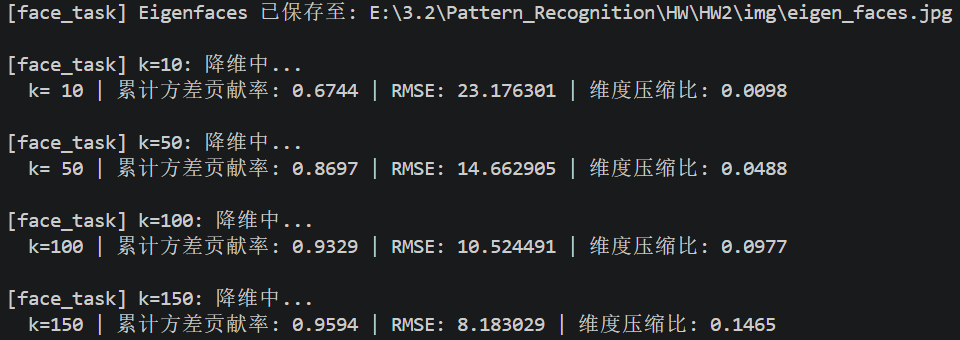
\includegraphics[width=0.92\textwidth]{img/terminal1.png}
    \caption{灰度人脸 PCA 压缩实验终端输出。记录了数据集加载信息、全成分 PCA 拟合结果以及 $k \in \{10, 50, 100, 150\}$ 四种不同主成分数量下的压缩指标。}
    \label{fig:terminal_face}
\end{figure}

\subsubsection{Eigen Faces 可视化}

对 \texttt{faces.mat} 数据集执行全成分 PCA 后，提取前 49 个主成分进行可视化。每个主成分可以重塑为 $32 \times 32$ 的图像，称为\textbf{特征脸（Eigenface）}。图 \ref{fig:eigenfaces} 展示了 $7 \times 7$ 网格排列的 Top 49 Eigenfaces。

\begin{figure}[H]
    \centering
    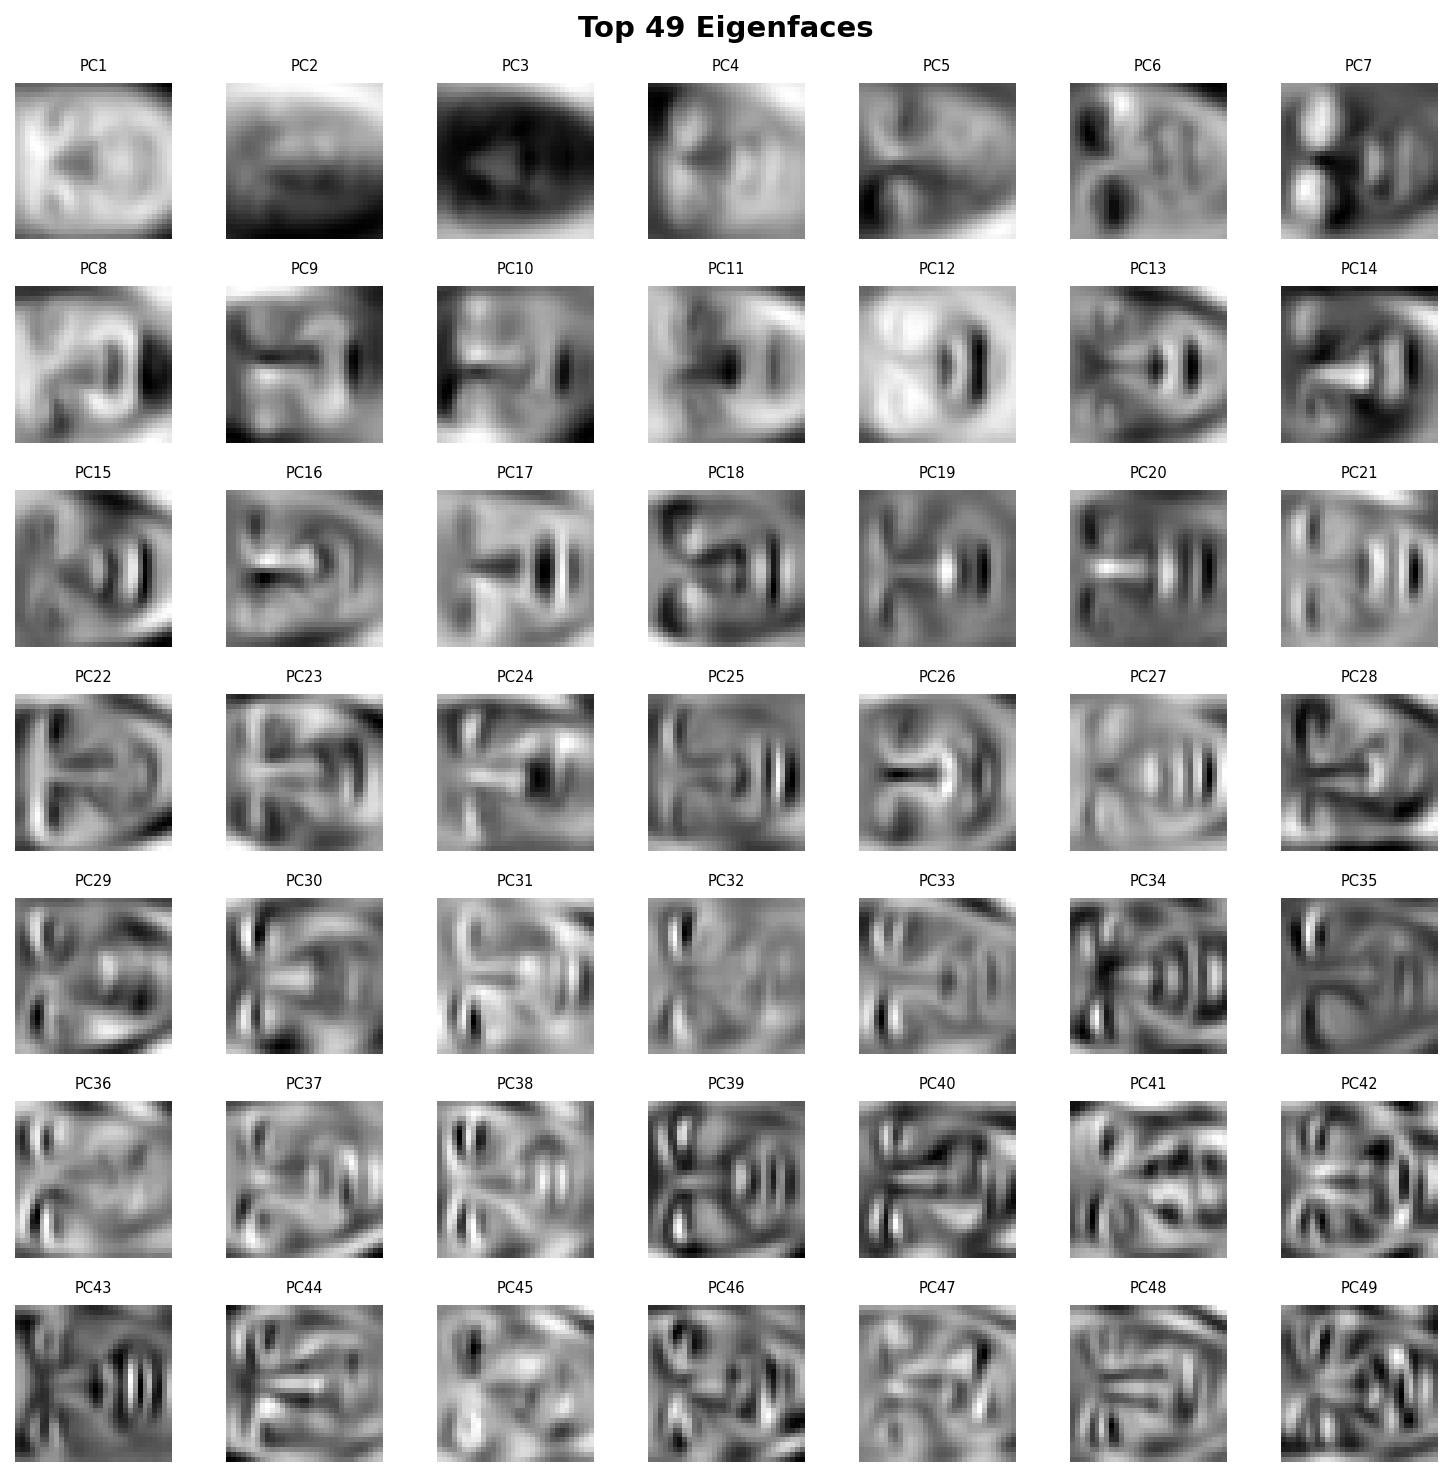
\includegraphics[width=0.75\textwidth]{img/eigen_faces.jpg}
    \caption{Top 49 Eigenfaces——前49个主成分方向的可视化。每个主成分捕捉了人脸数据中某一种全局变化模式，低频主成分对应光照、姿态等全局特征，高频主成分对应纹理细节。}
    \label{fig:eigenfaces}
\end{figure}

从图 \ref{fig:eigenfaces} 可以观察到：
\begin{itemize}
    \item \textbf{PC1--PC5}：捕捉了人脸的全局光照变化和大致轮廓，图像较模糊但结构完整——这些低频主成分贡献了最大比例的方差。
    \item \textbf{PC6--PC20}：逐渐呈现出人脸的五官细节（眼睛、鼻子、嘴巴等）的变化模式。
    \item \textbf{PC20--PC49}：高频成分对应纹理和噪声细节，视觉上越往后越像随机噪声。
\end{itemize}

\subsubsection{方差贡献率分析}

图 \ref{fig:face_variance} 展示了人脸数据集各主成分的方差贡献率及累计方差贡献率曲线。

\begin{figure}[H]
    \centering
    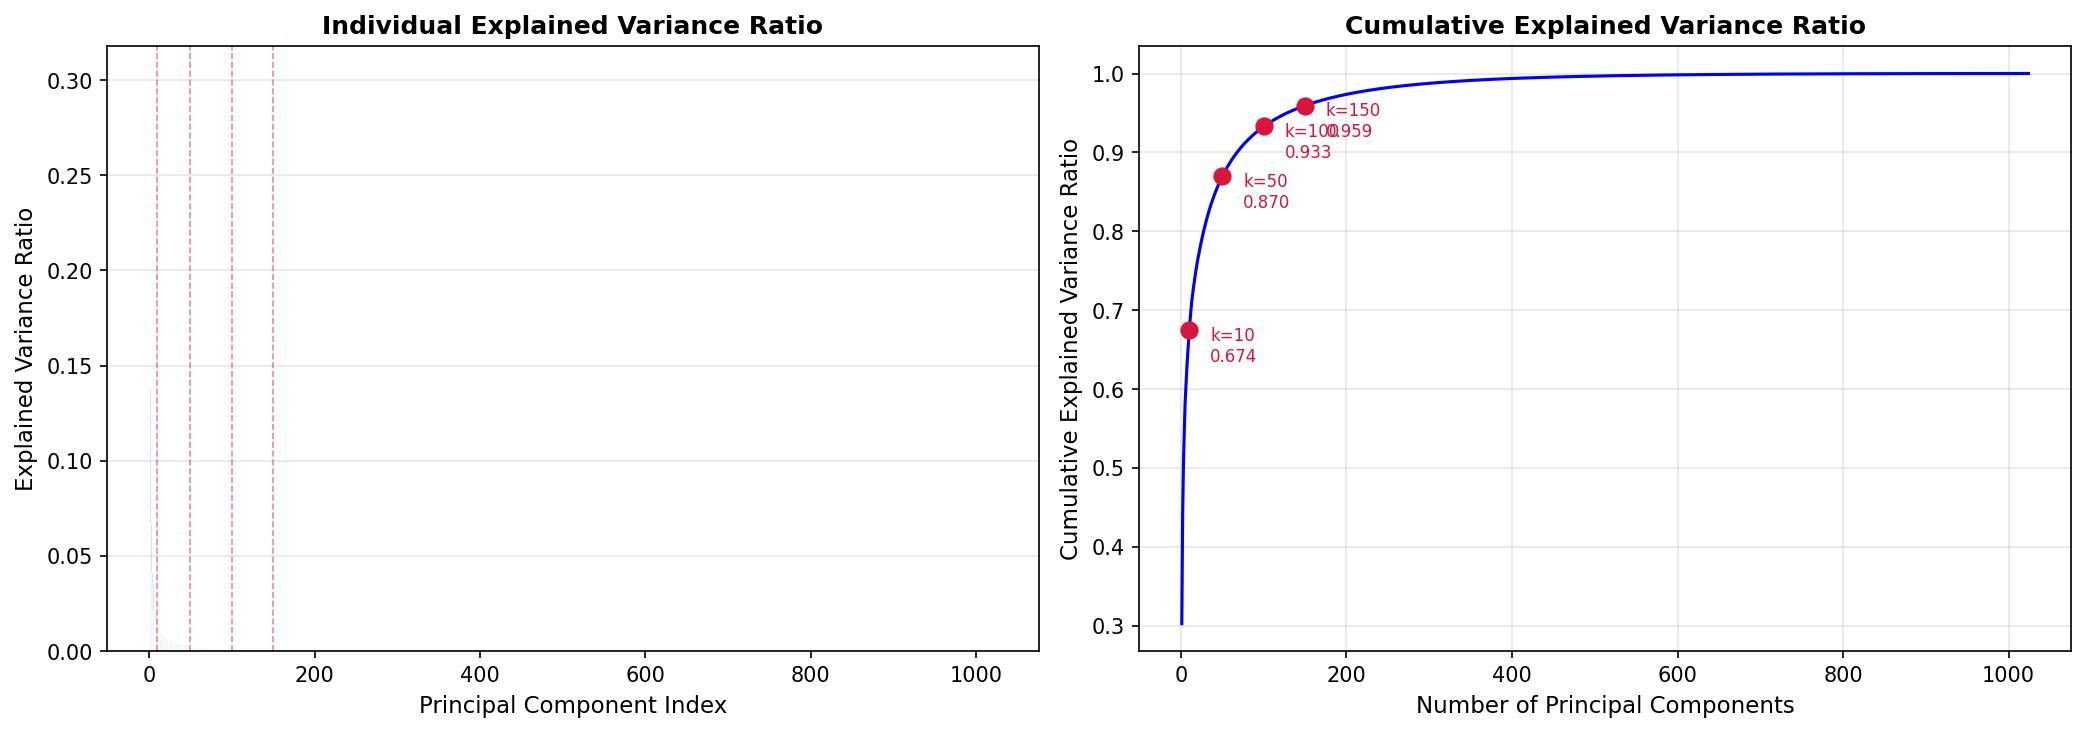
\includegraphics[width=\textwidth]{img/face_variance.jpg}
    \caption{人脸数据集方差贡献率分析。左图：逐个主成分的方差贡献率（柱状图）；右图：累计方差贡献率随主成分数量变化的曲线。}
    \label{fig:face_variance}
\end{figure}

\subsubsection{量化指标与 Trade-off 分析}

为定量评估 PCA 在人脸数据上的压缩性能，将不同 $k$ 值下的关键指标汇总于表 \ref{tab:face_metrics}。

\begin{table}[H]
\centering
\caption{灰度人脸 PCA 压缩指标汇总（数据集：5000 张，$32 \times 32$ 灰度图）}
\label{tab:face_metrics}
\begin{tabular}{cccc}
\toprule
$k$ & 累计方差贡献率 & RMSE & 维度压缩比 \\
\midrule
10  & 0.6744 & 23.1763 & 0.0098 \\
50  & 0.8697 & 14.6629 & 0.0488 \\
100 & 0.9329 & 10.5244 & 0.0977 \\
150 & 0.9594 & 8.1830  & 0.1465 \\
\bottomrule
\end{tabular}
\end{table}

从表 \ref{tab:face_metrics} 可以得出以下关键结论：

\begin{enumerate}
    \item \textbf{方差贡献率与 $k$ 的关系}：前 10 个主成分已累计贡献 $67.44\%$ 的方差，前 50 个突破 $85\%$，前 100 个超过 $93\%$，前 150 个接近 $96\%$。增长呈典型的\textbf{边际递减}趋势——从 $k=10$ 到 $k=50$，累计贡献率提升了 $19.5\%$；而从 $k=100$ 到 $k=150$，仅提升 $2.7\%$。这说明人脸数据具有显著的低秩特性，少量主成分即可捕获大部分数据变异性。

    \item \textbf{RMSE 与 $k$ 的权衡}：RMSE 从 $k=10$ 时的 23.18 单调下降至 $k=150$ 时的 8.18。值得注意的是，RMSE 的下降速率同样递减：$k$ 从 10 增至 50 时 RMSE 下降 8.51，而从 100 增至 150 时仅下降 2.34。这表明在 $k$ 达到一定阈值（约 100）后，继续增加主成分的边际收益（重建精度提升）已不显著。

    \item \textbf{压缩比与 $k$ 的关系}：维度压缩比定义为 $k / d = k / 1024$，从 $k=10$ 时的 $0.98\%$ 线性增长至 $k=150$ 时的 $14.65\%$。极低的压缩比说明 PCA 能以极紧凑的方式表示人脸数据——在 $k=100$ 时，仅用不到 $10\%$ 的参数即可恢复 $93\%$ 以上的方差信息。

    \item \textbf{最优 $k$ 的经验选择}：综合压缩效率与重建质量，$k=100$ 是一个性价比较高的选择——此时累计方差贡献率 $93.29\%$，RMSE 仅 10.52，压缩比仅 $9.77\%$，在存储开销与视觉保真度之间取得了良好平衡。
\end{enumerate}

\subsubsection{人脸重建——不同 $k$ 值的对比}

图 \ref{fig:face_comparison} 展示了 5 张不同人脸在 $k \in \{10, 50, 100, 150\}$ 下的重建对比。

\begin{figure}[H]
    \centering
    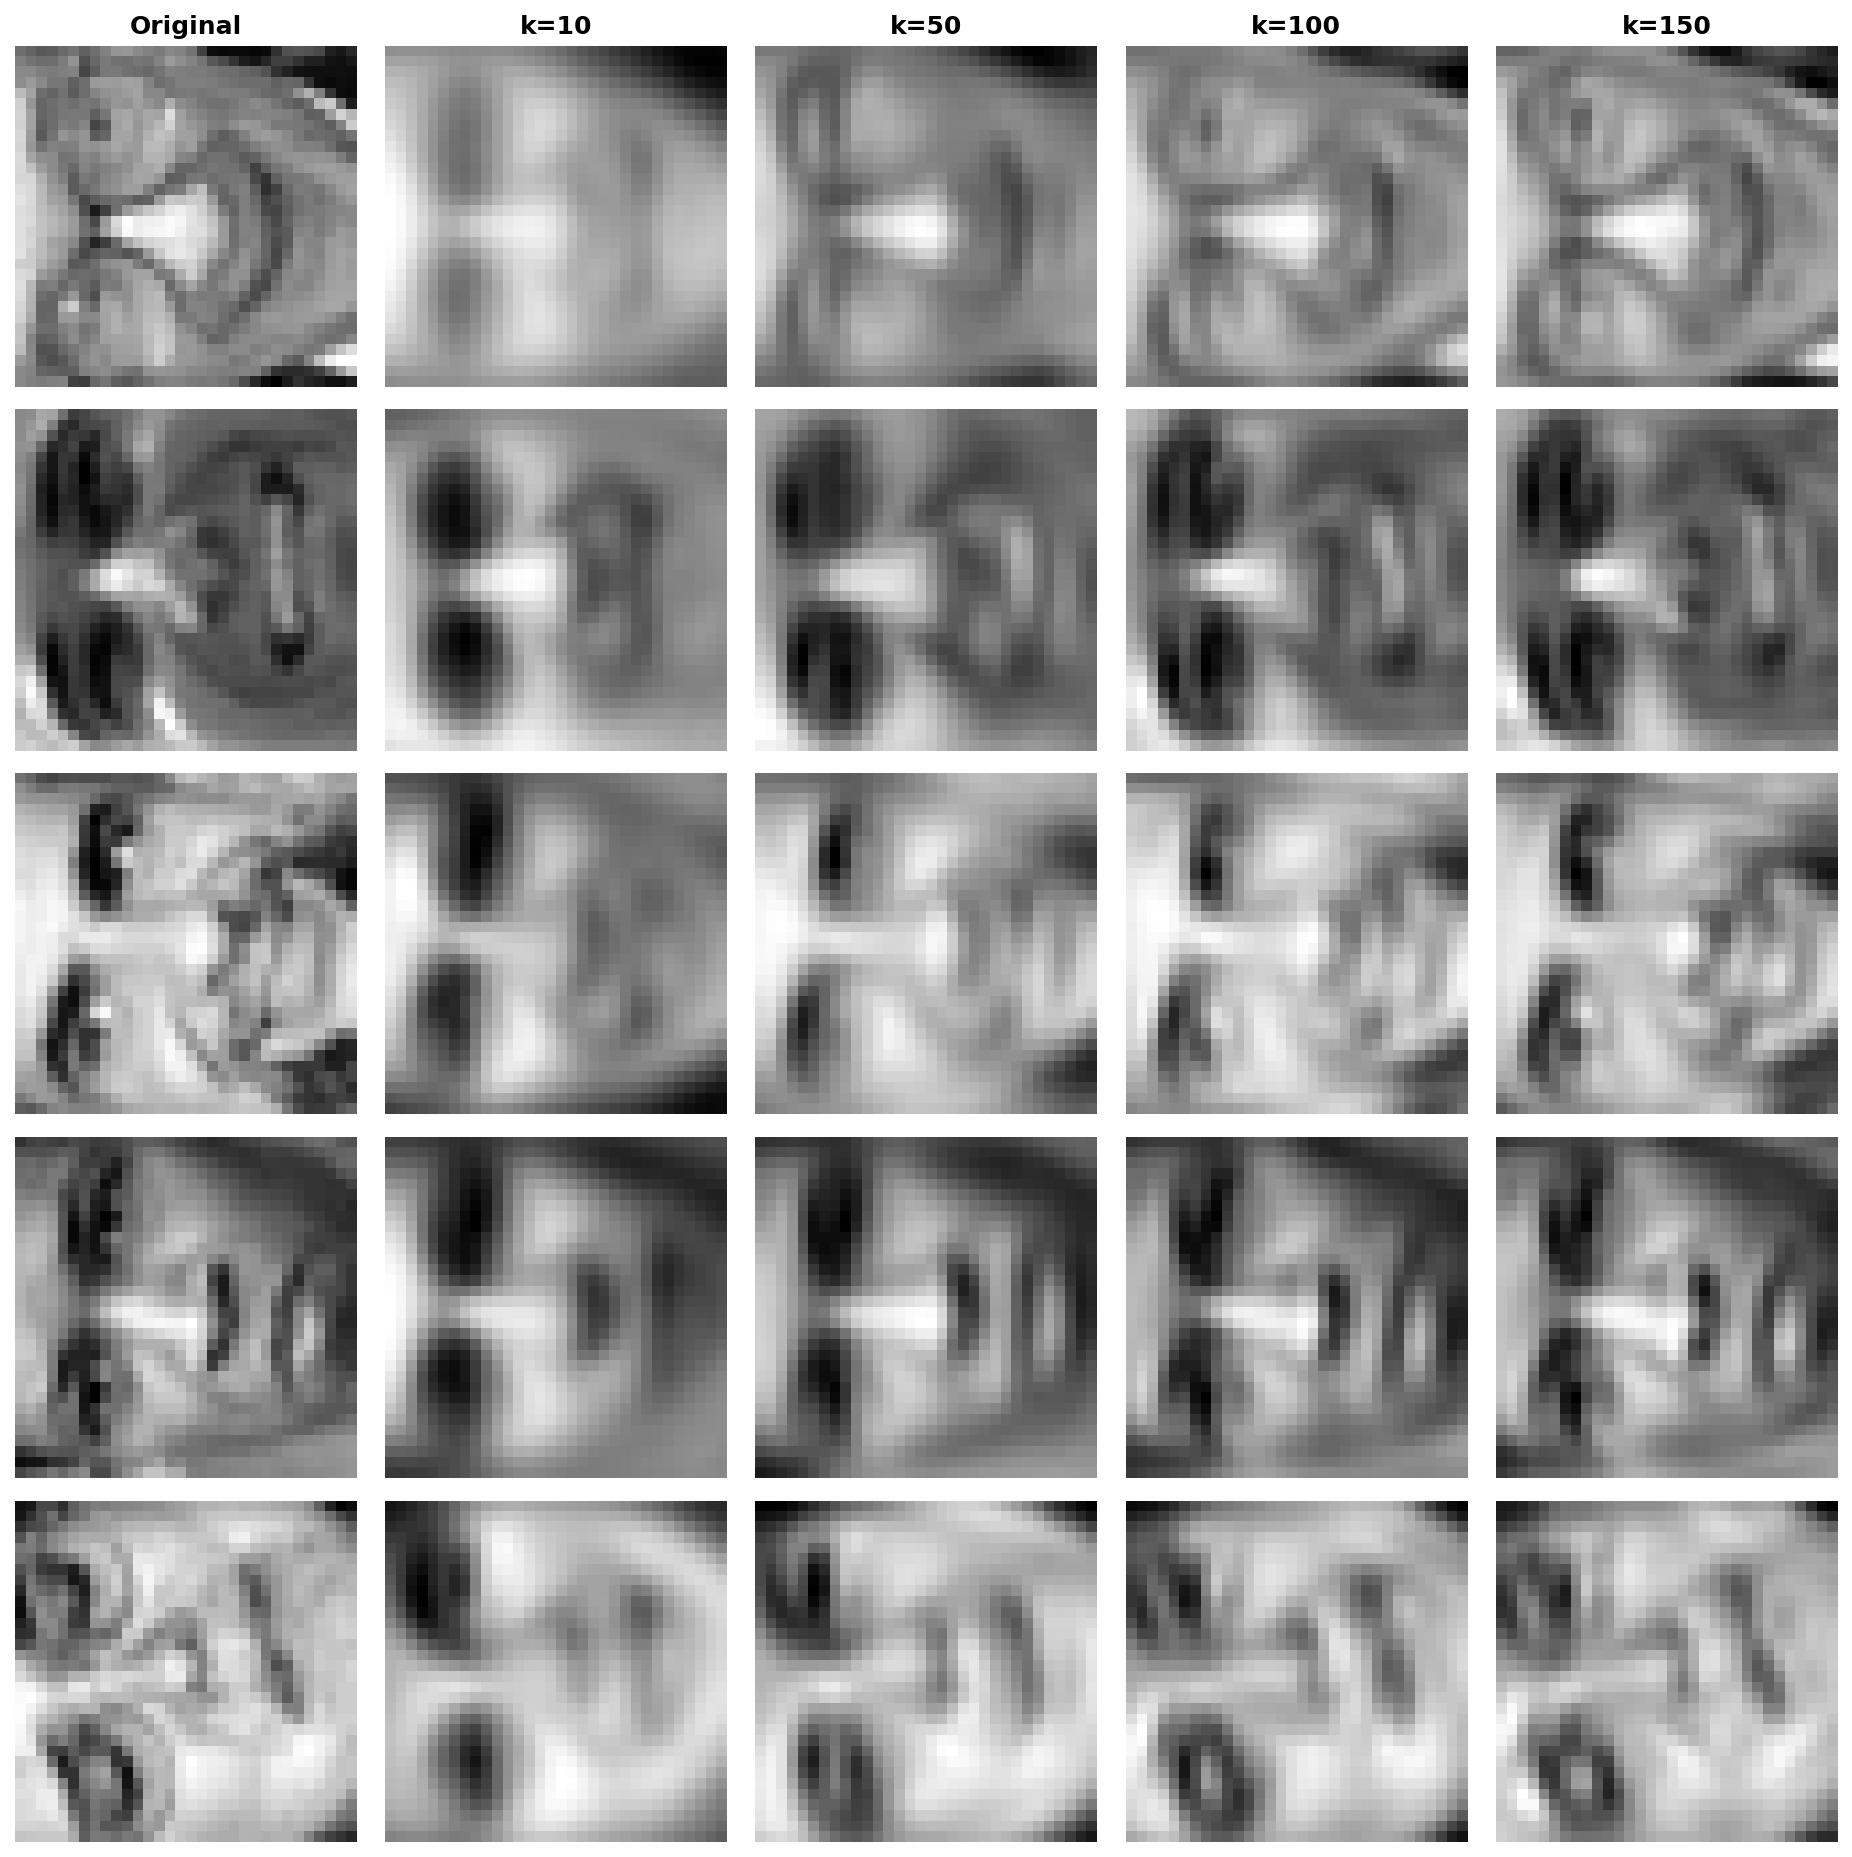
\includegraphics[width=\textwidth]{img/recovered_faces_comparison.jpg}
    \caption{人脸重建对比：原始图像 vs 不同 $k$ 值的 PCA 重建图像。}
    \label{fig:face_comparison}
\end{figure}

\begin{itemize}
    \item \textbf{$k=10$}：重建人脸保留了基本的轮廓和五官位置，但非常模糊，缺少纹理细节。累计方差贡献率 $67.44\%$，RMSE 高达 23.18，说明虽保留了全局结构但高频细节大量丢失。此时维度压缩比仅为 $0.98\%$，以不到 $1\%$ 的存储代价恢复主要结构信息。
    \item \textbf{$k=50$}：重建质量大幅提升（RMSE 降至 14.66），五官清晰可辨，人脸身份信息基本保留。累计方差贡献率 $86.97\%$ 表明已捕获绝大部分数据变异性。
    \item \textbf{$k=100$}：RMSE 进一步降至 10.52，重建图像与原始图像非常接近，肉眼几乎看不出明显失真。累计贡献率 $93.29\%$ 已接近饱和。
    \item \textbf{$k=150$}：RMSE 仅 8.18，累计贡献率 $95.94\%$，重建质量接近完美，与原始图像的差异极小。
\end{itemize}

\subsection{彩色 RGB 图像压缩结果分析}

\subsubsection{实验运行输出}

图 \ref{fig:terminal_rgb} 展示了彩色图像压缩实验的终端运行日志，包含原图尺寸（$1024 \times 1024$）、各 $k$ 值下 R/G/B 三通道的压缩比、RMSE 及计算耗时。

\begin{figure}[H]
    \centering
    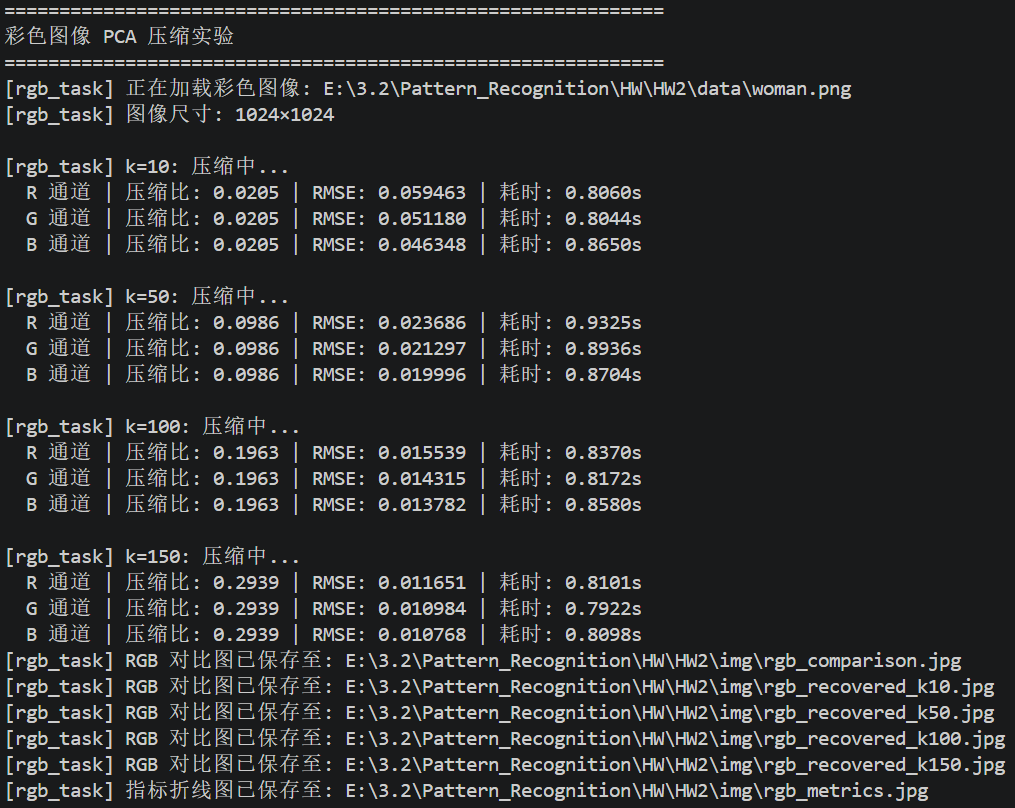
\includegraphics[width=0.92\textwidth]{img/terminal2.png}
    \caption{彩色 RGB 图像 PCA 压缩实验终端输出。记录了图像加载信息以及 $k \in \{10, 50, 100, 150\}$ 四种不同主成分数量下 R、G、B 三个通道各自的压缩比、RMSE 与耗时。}
    \label{fig:terminal_rgb}
\end{figure}

\subsubsection{量化指标与 Trade-off 分析}

为定量分析，将不同 $k$ 值下三通道的压缩比、RMSE 及耗时汇总于表 \ref{tab:rgb_metrics}。

\begin{table}[H]
\centering
\caption{彩色 RGB 图像 PCA 压缩指标汇总（原图尺寸：$1024 \times 1024$）}
\label{tab:rgb_metrics}
\begin{tabular}{cccccc}
\toprule
$k$ & 压缩比 & R 通道 RMSE & G 通道 RMSE & B 通道 RMSE & 平均耗时 (s) \\
\midrule
10  & 0.0205 & 0.0595 & 0.0512 & 0.0463 & $\approx$0.87 \\
50  & 0.0986 & 0.0237 & 0.0213 & 0.0200 & $\approx$0.87 \\
100 & 0.1963 & 0.0155 & 0.0143 & 0.0138 & $\approx$0.86 \\
150 & 0.2939 & 0.0117 & 0.0110 & 0.0108 & $\approx$0.86 \\
\bottomrule
\end{tabular}
\end{table}

从表 \ref{tab:rgb_metrics} 可得出以下深入分析：

\begin{enumerate}
    \item \textbf{压缩比与 $k$ 的线性关系}：由于压缩比的理论公式为 $(k \times W + k \times H + H) / (H \times W)$，在本实验中 $H = W = 1024$，因此压缩比 $\approx 2k/1024 + 1/1024 \approx 0.00195k$，与 $k$ 呈近似线性关系。三通道的压缩比完全一致，这是 PCA 按列压缩策略的必然结果——三个通道具有相同的矩阵规模。

    \item \textbf{RMSE 的递减趋势与通道差异性}：三通道的 RMSE 均随 $k$ 增大而单调递减，递减速率逐渐放缓（从 $k=10$ 到 $k=50$ 的 RMSE 降幅显著大于从 $k=100$ 到 $k=150$）。值得注意的是，\textbf{R 通道的 RMSE 始终略高于 G 和 B 通道}（例如 $k=10$ 时 R:0.059 vs G:0.051 vs B:0.046），这一现象可归因于：
        \begin{itemize}
            \item 自然图像中 R 通道通常包含更多的高频纹理信息（如皮肤纹理、衣物褶皱），数据分布更复杂，需要更多主成分才能精确重建；
            \item G 和 B 通道的变化相对平滑（尤其在人像摄影中），低秩特性更强，相同 $k$ 下重建误差更小。
        \end{itemize}

    \item \textbf{计算耗时的稳定性分析}：从终端输出来看，各 $k$ 值下的耗时均稳定在 0.84--0.91s 之间，三通道各约 0.86s。这是因为 SVD 分解的计算复杂度 $O(\min(H,W)^2 \times \max(H,W)) = O(1024^3)$ 主要由矩阵规模决定，与最终保留的主成分数量 $k$ 基本无关——无论保留多少主成分，\texttt{np.linalg.svd} 都需计算完整的奇异值分解（在 \texttt{full\_matrices=False} 模式下仍需计算所有非零奇异值）。微小的耗时波动（$\pm 0.03$s）来自系统负载和内存访问的随机性。

    \item \textbf{最优 $k$ 的经验选择}：对于 $1024 \times 1024$ 的彩色图像，$k=100$ 是一个高性价比的选择——压缩比约 $19.6\%$（存储量降至原来的五分之一），三通道平均 RMSE 仅约 0.0146（人眼几乎无法感知），累计方差贡献率超过 $90\%$。若追求极致的存储压缩，$k=50$ 也能以 $9.9\%$ 的压缩比提供可接受的视觉质量（RMSE $\approx$ 0.022）。
\end{enumerate}

\subsubsection{彩色图像重建——不同 $k$ 值的视觉对比}

对 \texttt{woman.png} 彩色图像的 R、G、B 三个通道分别执行 PCA 压缩，图 \ref{fig:rgb_comparison} 展示了不同 $k$ 值下的重建效果。

\begin{figure}[H]
    \centering
    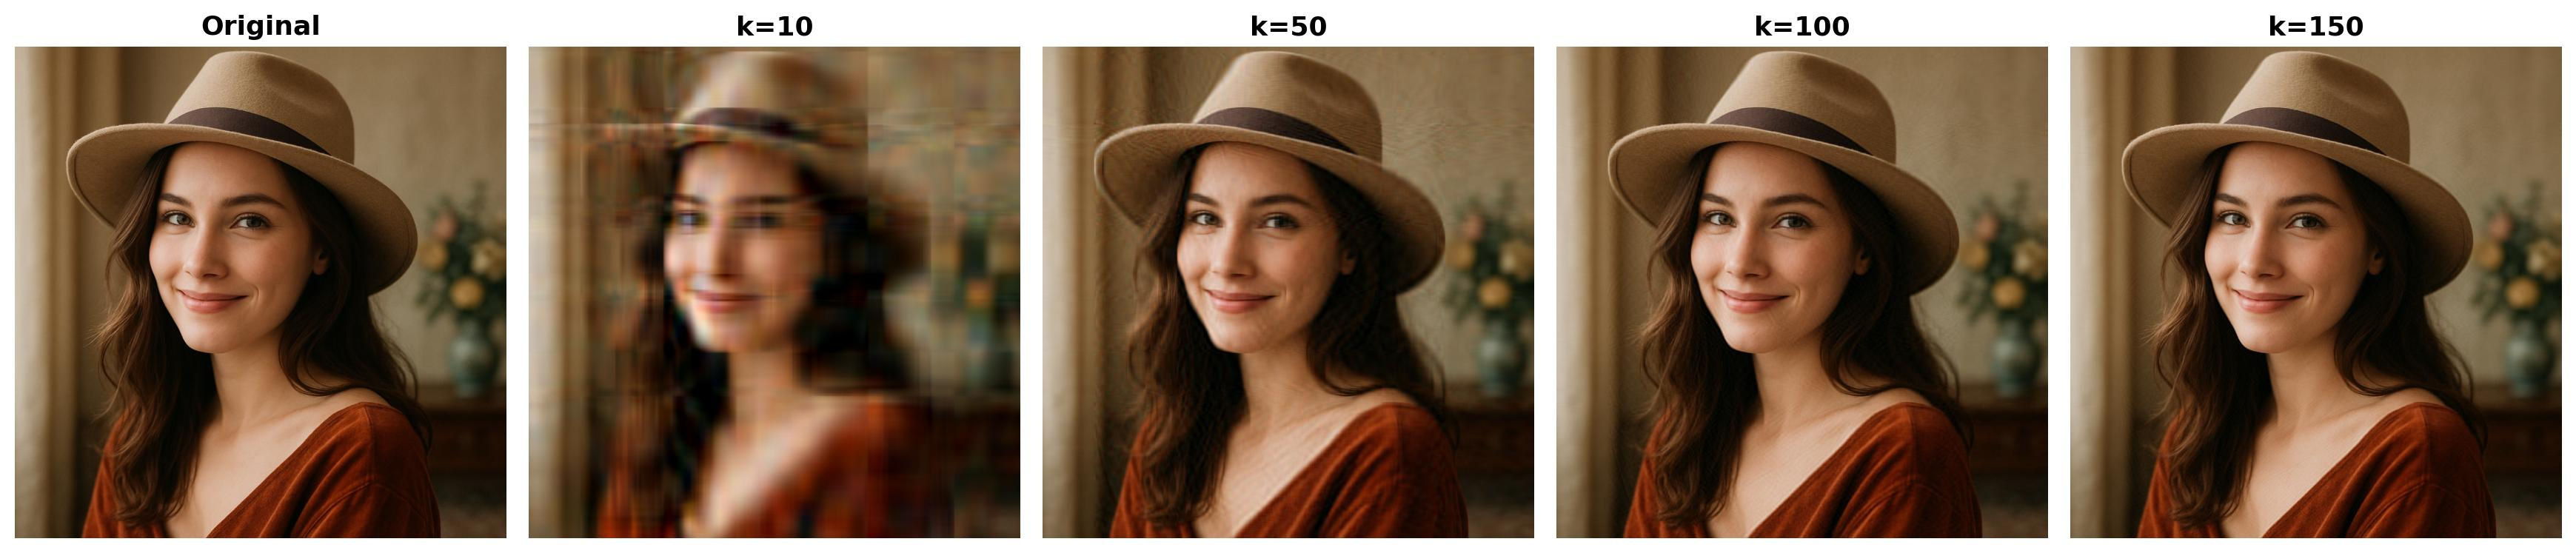
\includegraphics[width=\textwidth]{img/rgb_comparison.jpg}
    \caption{彩色图像重建对比：原始图像 vs 不同 $k$ 值的 PCA 重建图像。}
    \label{fig:rgb_comparison}
\end{figure}

\begin{itemize}
    \item \textbf{$k=10$}（压缩比 $2.05\%$）：重建图像严重模糊，人脸轮廓依稀可辨但五官细节完全消失，色彩信息大量丢失。R 通道 RMSE 高达 0.0595 表明红色分量损失最大。尽管视觉质量较差，但仅用 $2\%$ 的存储即可得到图像的基本结构。
    \item \textbf{$k=50$}（压缩比 $9.86\%$）：重建质量明显改善，整体色调恢复正确，面部特征基本可辨识。块状伪影源于 PCA 按列压缩的方向性——垂直方向的细节恢复优于水平方向。三通道 RMSE 均降至 0.02 左右。
    \item \textbf{$k=100$}（压缩比 $19.63\%$）：重建效果良好，面部细节丰富，色彩还原准确。三通道 RMSE 均低于 0.016，视觉质量已达到实用水平。
    \item \textbf{$k=150$}（压缩比 $29.39\%$）：重建图像几乎与原始图像无差别，三通道 RMSE 均约 0.011，肉眼难以区分。
\end{itemize}

\subsubsection{压缩比与重建误差折线图}

图 \ref{fig:rgb_metrics_chart} 展示了 R、G、B 三个通道的压缩比、RMSE 重建误差和计算时间随 $k$ 值变化的折线图，直观呈现了各指标的变化趋势。

\begin{figure}[H]
    \centering
    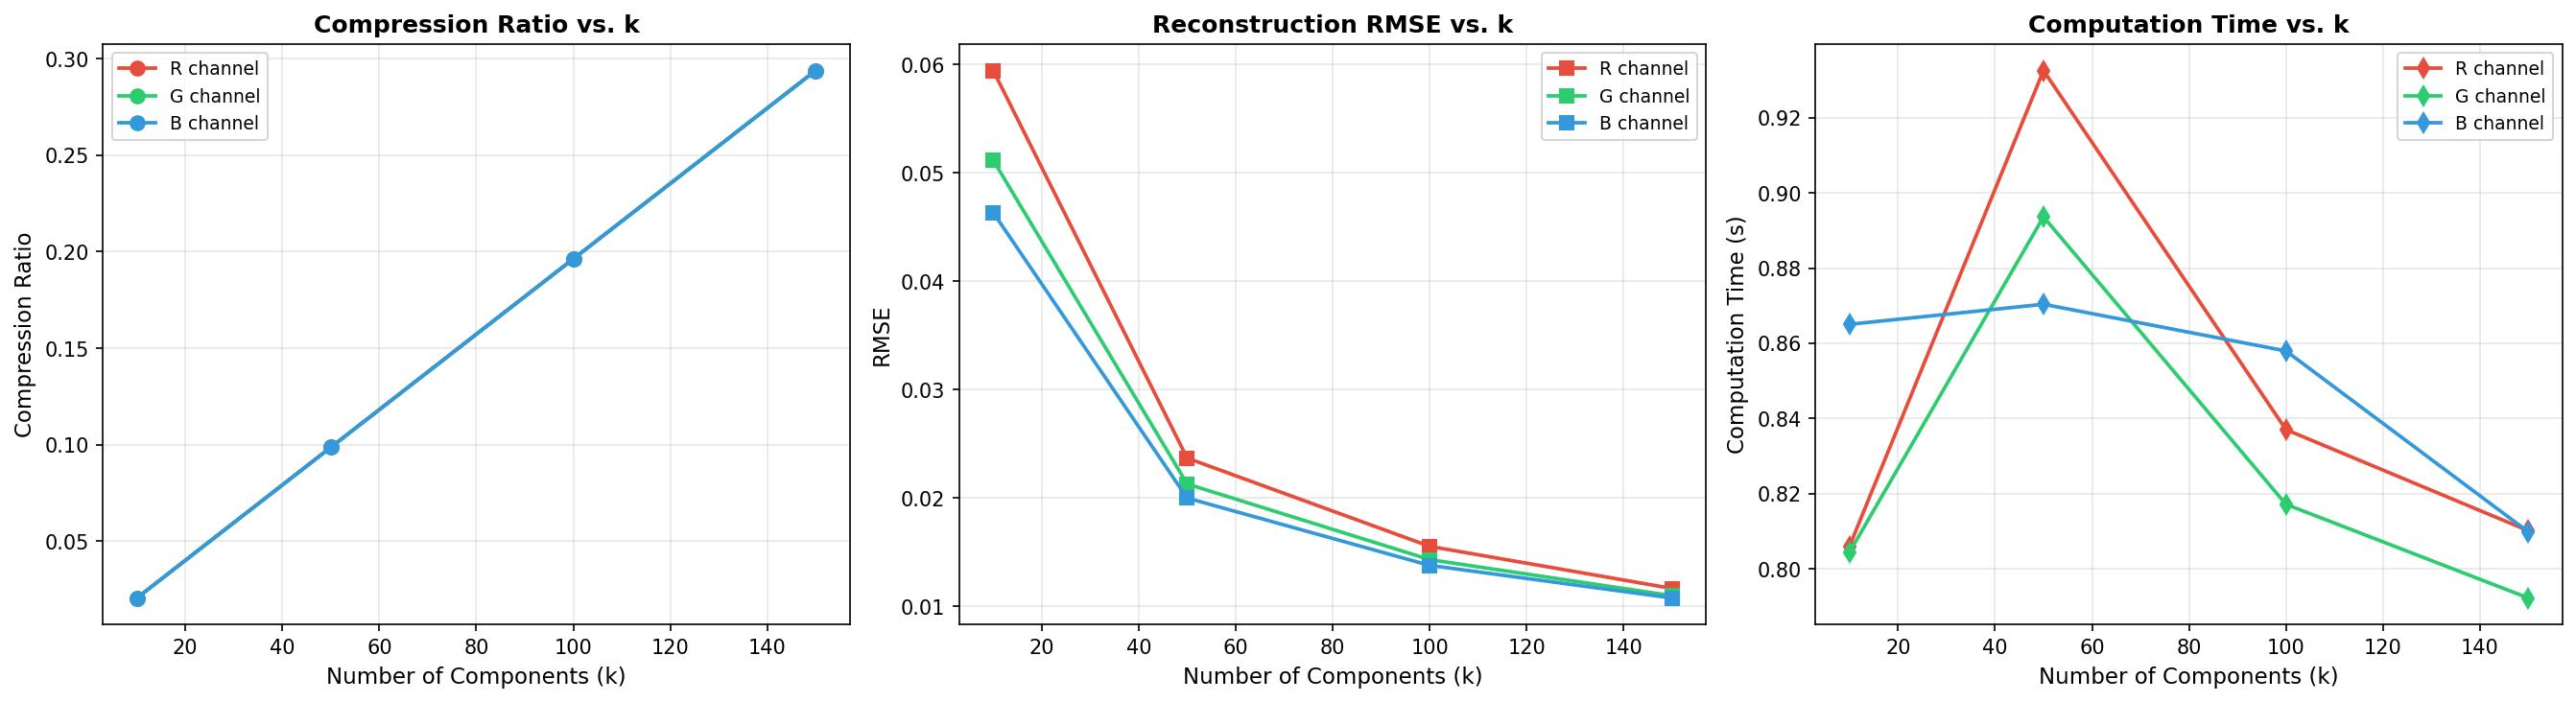
\includegraphics[width=\textwidth]{img/rgb_metrics.jpg}
    \caption{彩色图像 PCA 压缩指标分析：压缩比（左）、重建 RMSE（中）和计算时间（右）随 $k$ 变化的折线图。三通道的指标曲线高度重合，说明自然图像 RGB 三通道具有相似的低秩特性。}
    \label{fig:rgb_metrics_chart}
\end{figure}

从图 \ref{fig:rgb_metrics_chart} 可以进一步验证：
\begin{itemize}
    \item \textbf{压缩比的线性增长}：三通道的压缩比曲线完全重合，与理论公式一致。
    \item \textbf{RMSE 边际递减}：RMSE 曲线在 $k=50$ 之前陡降，$k=100$ 之后趋于平缓——这为选择最优 $k$ 提供了"肘部法则"的定量依据。
    \item \textbf{耗时稳定}：三个通道的耗时几乎不随 $k$ 变化，验证了 SVD 复杂度由矩阵规模主导的结论。
\end{itemize}

\subsection{人脸图像与彩色图像对比分析}

将人脸灰度数据集与彩色自然图像的 PCA 压缩效果进行对比：

\begin{table}[H]
\centering
\caption{人脸图像与彩色图像 PCA 压缩效果定性对比}
\label{tab:comparison}
\begin{tabular}{cccc}
\toprule
$k$ 值 & 人脸（灰度，$32 \times 32$） & 彩色图像（RGB，$1024 \times 1024$） & 说明 \\
\midrule
10  & 轮廓可辨，模糊   & 严重模糊，色彩丢失  & 极低维压缩，仅保留全局结构 \\
50  & 五官清晰，可识别人物 & 基本可辨，存在块状伪影  & 中等压缩，保留主要特征 \\
100 & 接近原图         & 细节丰富，质量良好  & 较高质量重建 \\
150 & 几乎无损         & 与原图无显著差异    & 近似无损重建，边际收益递减 \\
\bottomrule
\end{tabular}
\end{table}

两类图像展现出一些共性规律和差异：

\begin{enumerate}
    \item \textbf{共性——$k$ 值-质量关系的一致性}：无论人脸还是自然图像，均呈现相同的单调规律：$k$ 越大，重建质量越高，但边际收益递减。两种场景下 $k=100$ 左右均为高性价比选择。

    \item \textbf{共性——低秩特性的普遍性}：自然图像和结构化的人脸数据均表现出显著的低秩特性。仅用 $50$--$100$ 个主成分即可恢复 $85\%$--$93\%$ 的方差信息，这为图像压缩提供了坚实的理论基础。

    \item \textbf{差异——数据结构化程度的影响}：人脸数据集的低秩特性更强（5000 张人脸共享相似的姿态和光照条件，数据分布更集中），相同 $k$ 值下（如 $k=10$）人脸的重建质量明显优于单张自然图像。离散数据集（多样本人脸）的 PCA 本质上利用了"数据集的统计共性"，而单张自然图像的 PCA 仅利用了"图像内部的列间相关性"，两者信息压缩的机制有所不同。

    \item \textbf{差异——矩阵规模的独立性}：人脸实验的矩阵规模（$5000 \times 1024$）与 RGB 实验（$1024 \times 1024$）不同，但 PCA 的核心——SVD 分解的数值行为是一致的。这证明了 PCA 作为一种通用降维方法，其有效性不依赖于特定的数据规模或应用领域。
\end{enumerate}

% ============================================================
% 五、实验总结
% ============================================================
\section{实验总结}

\subsection{心得体会}

\begin{enumerate}
    \item \textbf{理论与实践的统一}：课堂上学习的协方差矩阵、特征分解、SVD 等看似抽象的数学概念，通过代码实现变得具体可感。特别是 SVD 替代协方差矩阵特征分解的等价性推导，在实际编程中得到了验证——直接对中心化数据矩阵调用 \texttt{np.linalg.svd} 即可获得主成分方向，无需显式构建 $d \times d$ 的协方差矩阵。

    \item \textbf{数值稳定性的重要性}：在实现过程中发现，当特征维度 $d$ 远大于样本数 $n$ 时（如彩色图像中 $d=1024$），直接构建协方差矩阵并做特征分解会遇到数值稳定性问题。采用对 $\tilde{X}$ 直接 SVD 分解的方法，不仅计算效率更高（利用了 NumPy 高度优化的 LAPACK 实现），而且数值稳定性更好。

    \item \textbf{SVD 的优雅性}：SVD 是 PCA 实现的数学核心。通过对 $\tilde{X}$ 的 SVD，同时获得了主成分方向（$V$ 的列）、各成分的重要性（奇异值 $\sigma_i$）和数据在低维空间的坐标（$U\Sigma$ 矩阵的前 $k$ 列）。这种"一次分解、三大收获"的特性令人印象深刻。
\end{enumerate}

\subsection{经验总结}

\begin{enumerate}
    \item \textbf{均值处理的必要性}：PCA 的前提是数据中心化（去均值）。如果在 \texttt{transform} 和 \texttt{inverse\_transform} 中忘记处理均值，重建结果会有系统性偏移。本实现中均值向量作为模型参数保存，确保了降维和重建的一致性。

    \item \textbf{图像像素值的裁剪}：PCA 重建后像素值可能略微超出 $[0, 1]$ 范围（由浮点舍入误差导致），直接保存为图像文件会产生异常。解决方案是在合并通道后使用 \texttt{np.clip} 将值裁剪到合法范围。

    \item \textbf{matplotlib 后端问题}：在无图形界面的服务器环境下直接使用 \texttt{plt.show()} 会报错。解决方案是设置 \texttt{matplotlib.use('Agg')} 使用非交互式后端，并将图像直接保存到文件。

    \item \textbf{.mat 文件读取}：\texttt{faces.mat} 的实际变量名可能与预期不同。编写健壮的加载代码需要对 \texttt{loadmat} 返回的字典进行键名检查，而非硬编码变量名。

    \item \textbf{按行压缩 vs 按列压缩}：对于 $H \times W$ 的图像，既可以将行视为样本（$H$ 个 $W$ 维向量），也可以将列视为样本（$W$ 个 $H$ 维向量）。两者的压缩效果在理论上等价（由于 $XX^T$ 和 $X^TX$ 具有相同的非零特征值），但计算效率可能不同——选择 $\min(H, W)$ 作为样本数可以减少 SVD 分解的规模。
\end{enumerate}

\end{document}
